\documentclass[10pt,letterpaper]{article}
\usepackage[top=0.85in,left=2.75in,footskip=0.75in]{geometry}
\usepackage{amsmath,amssymb}
\usepackage{changepage}
\usepackage{textcomp,marvosym}
\usepackage{cite}
\usepackage{nameref,hyperref}
\usepackage[right]{lineno}
\usepackage[nopatch=eqnum]{microtype}
\DisableLigatures[f]{encoding = *, family = * }
\usepackage[table]{xcolor}
\usepackage{array}
\usepackage{graphicx}
\usepackage{epstopdf}
\usepackage{longtable}
\usepackage{booktabs}
\usepackage{calc}
\usepackage{soul}
\usepackage[normalem]{ulem}
\usepackage{lastpage,fancyhdr}
\usepackage[aboveskip=1pt,labelfont=bf,labelsep=period,justification=raggedright,singlelinecheck=off]{caption}
\renewcommand{\figurename}{Fig}
\graphicspath{{./media/}}
% Working merge file: base = current PLOS_article.tex, donor = Try1.tex for lost text/formulas.
\newif\iflocalfigurepreview
\localfigurepreviewtrue
\bibliographystyle{plos2025}
\makeatletter
\renewcommand{\@biblabel}[1]{\quad#1.}
\makeatother
\pagestyle{fancy}
\fancyhf{}
\rfoot{\thepage/\pageref{LastPage}}
\renewcommand{\headrulewidth}{0pt}
\renewcommand{\footrule}{\hrule height 2pt \vspace{2mm}}
\fancyheadoffset[L]{2.25in}
\fancyfootoffset[L]{2.25in}
\lfoot{\today}
\raggedright
\setlength{\parindent}{0.5cm}
\setlength{\emergencystretch}{3em}
\textwidth 5.25in
\textheight 8.75in
\begin{document}
\vspace*{0.2in}
\begin{flushleft}
{\Large
\textbf{An adaptive hybrid model for wildfire front forecasting based on cellular automata, multi-agent UAV observations, and binary data assimilation: A case study of the 2021 Dixie Fire}
}
\newline
\\
Ramazan Sadvakassov\textsuperscript{1},
Kuralay Sadvakassova\textsuperscript{1,2*},
Bijeesh Kozhikkodan Veettil\textsuperscript{3,4*},
Nurzada Amangeldy\textsuperscript{1},
Altynbek Sharipbay\textsuperscript{1},
Assel Zhumabayeva\textsuperscript{1},
Dzhavdet Suleymanov\textsuperscript{5}
\\
\bigskip
\textbf{1} Faculty of Information Technologies, L.N. Gumilyov Eurasian National University, Astana 010008, Kazakhstan
\\
\textbf{2} Astana IT University, Astana, Kazakhstan
\\
\textbf{3} Laboratory of Ecology and Environmental Management, Science and Technology Advanced Institute, Van Lang University, Ho Chi Minh City, Vietnam
\\
\textbf{4} Faculty of Applied Technology, Van Lang School of Technology, Van Lang University, Ho Chi Minh City, Vietnam
\\
\textbf{5} Institute of Applied Semiotics, Tatarstan Academy of Sciences, Kazan, Russian Federation
\\
\bigskip
* Correspondence: k.sadvakassova@astanait.edu.kz; bkozhikkodanveettil@vlu.edu.vn
\\
\textbf{Short title:} Hybrid CA+MAS wildfire front forecasting
\end{flushleft}
\section*{Abstract}
This study presents a retrospective case-study evaluation of a hybrid framework for daily wildfire-front forecasting during the 2021 Dixie Fire in California, USA. The framework couples a stochastic cellular automaton (CA) with a multi-agent system (MAS) of simulated UAV observations and a lightweight binary data-assimilation scheme. The model uses topography, vegetation, fuel proxies, and meteorological forcings derived from Copernicus GLO-30/SRTM, ESA WorldCover, MODIS NDVI, MODIS burned-area products, VIIRS active-fire detections, and ERA5-Land data. The CA produces a daily forecast of wildfire evolution, while the MAS directs a configurable set of simulated aerial agents toward spatially distributed high-information regions identified from predicted growth and fire-front structure. Agent observations are assimilated through a binary confirm-deny update that suppresses false ignitions and restores missed burning cells before the next forecast step; the observed footprint can also support local blending of daily weather fields before propagation resumes. In the verified evaluation window from 14 to 18 August 2021, with corrected road and water barrier masks enabled in the CA component, the hybrid CA+MAS framework increased the mean Intersection over Union (IoU) from 0.6664 for the standalone baseline CA to 0.6992, corresponding to an absolute gain of 0.0328, while the mean F1 score increased from 0.7998 to 0.8229. These findings indicate that targeted recurrent aerial observations can improve short-horizon wildfire-front reconstruction while preserving the computational simplicity and interpretability of the underlying cellular automaton.

\noindent\textbf{Keywords:} wildfire front forecasting, wildfire spread, cellular automaton, multi-agent system, unmanned aerial vehicle, data assimilation

\clearpage
\newgeometry{top=0.85in,left=1in,right=1in,footskip=0.75in}
\linenumbers
\section*{Introduction}

Wildfires are increasingly recognized as a systemic environmental and
societal risk because they threaten public health, critical
infrastructure, ecosystems, and evacuation safety. Recent studies
indicate that climate-driven drought, heat extremes, and strong winds
are lengthening fire-season duration and expanding the spatial extent of
fire-prone conditions, which increases the need for timely and
interpretable forecasting tools \cite{jolly2015,shaik2025}.

These demands are especially acute in the wildland-urban interface
(WUI), where rapidly changing wildfire front behavior can affect
exposure, suppression priorities, and evacuation planning. However,
strong wind shifts, heterogeneous fuel conditions, and local topographic
effects are not unique to the WUI; they complicate wildfire spread
forecasting more broadly and make static fire-spread estimates quickly
outdated.

Existing wildfire modeling approaches address different parts of this
problem but rarely combine speed, physical interpretability, and
adaptive observation. Fire Area Simulator (FARSITE) and Prometheus, the
Canadian Wildland Fire Growth Simulation Model, provide interpretable
fire-spread simulations, but they require careful data preparation and
can be demanding in operational settings \cite{finney1998,tymstra2010}. Remote-sensing and
machine-learning approaches can extract useful spatiotemporal patterns
from satellite products, but they often depend on large training
datasets and may offer limited interpretability in rapidly evolving
wildfire environments \cite{chuvieco2020,andrianarivony2024}.

Observation-informed wildfire forecasting has also been explored using
satellite-derived fire progression products and data-assimilation
schemes that update model states with newly available observations
\cite{cheng2022,mcclure2023,chen2022}. These studies support the value
of closed-loop forecast updating, but they do not remove the practical
need for computationally lightweight and interpretable forecasting
frameworks.

This gap motivates a closed-loop forecasting framework in which a
physically interpretable spread model is updated with targeted
observations. In this study, the forecasting target is daily wildfire
front progression. We couple a stochastic cellular automaton (CA) with a
multi-agent system (MAS) of simulated unmanned aerial vehicle (UAV)
observers that are directed toward informative regions of the predicted
fire front. The CA represents the daily evolution of the wildfire front
as a function of terrain, vegetation, fuel proxies, and meteorological
forcing, while the MAS supplies localized observations that are
assimilated before the next forecast step.

The empirical framework combines satellite-derived observational products
with reanalysis forcing data at a daily simulation time step. MODIS
burned-area and VIIRS active-fire products are used as observational
constraints and evaluation references, whereas ERA5-Land is used as
meteorological forcing rather than as direct fire observation. Static
spatial inputs include topography, land-cover-derived fuel proxies,
vegetation condition, and barrier layers.

Rather than claiming a universal operational system, this work presents
a retrospective case-study evaluation of an interpretable hybrid CA+MAS
framework for the 2021 Dixie Fire in California, USA. The novelty lies
in combining an explicit daily
wildfire-front CA forecast, informative-region UAV tasking, and a
lightweight binary assimilation rule within one reproducible framework.
The following sections review related approaches, describe the data and
methodology, and evaluate the framework against observed wildfire
dynamics.

\section*{Overview of existing approaches and their limitations}

\subsection*{Cellular automata and physics-based wildfire spread models}

One of the most common approaches to modeling the spatial dynamics of
forest fires is cellular automata (CA), in which the landscape is
represented as a grid of cells that transition between discrete
states---\emph{burning}, \emph{burned}, and \emph{unburned}---depending on the state of
neighboring cells and a defined set of rules. This method allows
consideration of topography, fuel combustibility, wind, and other
spatial factors, providing a balance between computational simplicity
and realism.

An example of a modern solution is HexFire, which uses a hexagonal grid
in which all nearest neighbors are equidistant, reducing the anisotropy
of fire spread. The model requires only a small parameter set and a few
core input maps, such as fuel combustibility, wind speed, and wind
direction, while simulating spread through both direct contact and ember
transport \cite{schumaker2022}. Cellular automata can be deterministic
or stochastic, and adaptive cellular-automaton variants have also been
used to represent abrupt spread changes under strong wind conditions
\cite{freire2019}.

Physics-based models, particularly
advection--diffusion--reaction (ADR) formulations, provide a more
detailed description of combustion processes based on conservation laws
for energy and mass. These models account for fuel moisture, radiation,
topography, and air movement \cite{navasmontilla2025}. In this family of
approaches, ignition and spread depend on interacting physical terms,
whereas radiative effects are commonly represented through nonlinear
temperature-dependent transport terms.

Related coupled-model studies also examine wildfire spread near
populated areas, where interactions among spread dynamics, built
environments, and suppression constraints become especially important
\cite{szasdi2025}.

\subsection*{Mapping combustible materials using artificial
intelligence}

Accurate assessment of the types and distribution of combustible
materials is a critical component of fire modeling and forecasting. The
integration of remote-sensing data with machine-learning algorithms
plays a key role in this process.

A modern example is the FuelVision system, which uses multispectral,
radar, and topographic predictors to construct fuel maps
\cite{shaik2025}. In that line of work, ensemble learning and related
data-fusion strategies are used to improve mapping robustness when
field observations are sparse or class distributions are imbalanced.
Related studies also note that synthetic-sample generation and
post-processing with vegetation indices can help stabilize fuel-class
mapping when field reference data are limited, especially for
distinguishing non-burnable classes from combustible vegetation.

More broadly, combining remote-sensing products with modern
machine-learning workflows can improve the reliability and scalability
of combustible-material mapping, thereby providing a stronger input base
for physical, mathematical, and stochastic fire-spread models.

\subsection*{Deep learning-based fire spread prediction}

Deep-learning methods have expanded the range of data-driven
spatiotemporal wildfire-prediction approaches.

Convolutional neural networks (CNNs) are used to extract spatial
features from satellite data, enabling the detection of active fires and
the direction of the fire front. Multi-kernel CNN designs have been
used to better account for landscape heterogeneity in next-day spread
prediction tasks \cite{marjani2023}.

Review literature also reports recurrent and attention-based models for
capturing temporal fire evolution and longer-range spatial dependencies
in satellite-driven wildfire prediction tasks \cite{andrianarivony2024}.
In particular, ConvLSTM-style architectures and hybrid
attention-augmented recurrent models are used to combine spatial fire
patterns with short-term temporal evolution, thereby extending purely
frame-based prediction toward sequence-aware spread forecasting.

Transformer architectures have also been explored to model longer-range
spatiotemporal dependencies in wildfire prediction \cite{andrianarivony2024}.

\subsection*{Multi-agent systems and autonomous control}

Modern forest fire monitoring and suppression tasks require not only
accurate models but also rapid, coordinated action. This is where
multi-agent systems (MAS), reinforcement learning, and multi-agent
reinforcement learning play an important role.

Recent reviews highlight that autonomous UAV platforms can support fire
detection, mapping, navigation, and decision support, while conceptual
drone-swarm systems have been proposed for coordinated suppression and
front monitoring in rapidly evolving wildfire environments
\cite{partheepan2023,ausonio2021}.

Related benchmark and simulation studies also explore coordinated
multi-agent wildfire response in more explicitly heterogeneous settings,
including scenarios with firefighters, aerial agents, and ground
equipment trained or evaluated under shared resource constraints
\cite{ramadan2024,partheepan2023}.

In addition to software simulators, physical platforms based on the
Internet of Things and UAVs are being actively developed for early
detection and targeted firefighting \cite{ramadan2024}. These integrated sensing
architectures are relevant here because they emphasize rapid
observation, communication, and local situational updating rather than
stand-alone spread prediction alone.

Other studies discuss swarm-coordination strategies such as belief-space
planning for distributed autonomous sensing \cite{ausonio2021}. Although
these methods are not implemented in the present manuscript, they help
frame the broader literature context in which coordinated observation
and task allocation are treated as coupled problems.

Taken together, the reviewed studies indicate a persistent trade-off:
no single family of methods simultaneously provides interpretable fire
spread dynamics, efficient computation over large domains, and adaptive
state updating under rapidly changing conditions
\cite{freire2019,schumaker2022,navasmontilla2025,andrianarivony2024,marjani2023,partheepan2023,ausonio2021,ramadan2024}.

Models based on cellular automata (CA) are easy to implement and can
reproduce the spatial dynamics of a fire, considering local factors such
as topography, fuel, and wind \cite{freire2019,schumaker2022}, but they are sensitive to parameter settings and lack
built-in mechanisms for real-time data updates, limiting their
applicability in operational scenarios. Physical-mathematical
advection-diffusion-reaction (ADR) models provide a more detailed
description of combustion processes, including fuel moisture, radiation,
and air movement \cite{navasmontilla2025}, but their practical
use in online forecasting is limited by high computational complexity
and reliance on numerous input parameters. Deep learning models have
shown strong performance for predicting fire spread based on satellite
data, particularly when employing CNNs, convolutional long short-term
memory (ConvLSTM) networks, and transformer architectures
\cite{andrianarivony2024,marjani2023}, but these models require substantial
amounts of labeled data, are not always physically interpretable, and
often fail to account for dynamic real-world environmental factors.
Multi-agent systems (MAS) and reinforcement-learning-based
solutions show promise for autonomous fire response and suppression
tasks \cite{partheepan2023,ausonio2021,ramadan2024}. Scenarios involving
heterogeneous agents such as drones, bulldozers, and firefighters enable
the simulation of coordinated collective actions. Nevertheless, the
effectiveness of these systems is largely determined by the accuracy of
the underlying environmental model and the reliability of input data
\cite{ramadan2024}.

This gap motivates the hybrid computational architecture adopted in the
present study. The CA component serves as the base spread model,
simulating fire propagation while accounting for topography,
vegetation, humidity, and meteorological factors, thereby preserving
physical interpretability and stability \cite{schumaker2022}. The MAS
component is represented here by a simulated UAV observation layer that
supplies targeted observations for retrospective data assimilation
rather than by real deployed aircraft. The resulting closed loop of
forecast, target selection, observation, and state updating is designed
to retain the transparency of CA-based wildfire modeling while adding
the adaptive observation logic that is often missing from stand-alone
spread models.

\section*{Materials and methods}

The proposed integrated framework combines a cellular automaton for
daily fire-front propagation with a simulated drone observation layer
used in retrospective evaluation. The system architecture is organized
so that the spread model generates a daily forecast, the drone layer is
assigned toward informative fire-front regions, and the collected
observations are assimilated back into the model before the next
forecast step.

This design is operationally motivated but evaluated here only in a
retrospective replay setting: the CA forecast acts as the predictive
backbone, while the simulated observation layer provides localized
state corrections that can be examined without claiming historical live
UAV deployment during the 2021 event.

The CA and MAS components are coupled through a lightweight binary
assimilation module that applies explicit cell-level corrections to the
current fire state. This configuration supports daily updates across a
large raster domain while suppressing spurious ignitions, restoring
missed burning cells, and improving delineation of the fire front.

\iflocalfigurepreview
\begin{minipage}{\linewidth}
\centering

\includegraphics[width=6.0in,height=4.8in,keepaspectratio]{fig1_workflow.png}
\captionsetup{hypcap=false}
\captionof{figure}{\textbf{Closed-loop workflow of the retrospective CA+MAS wildfire
forecasting framework.} The sequence runs from multi-source data
preparation and daily CA spread prediction to informative-region
selection, drone-task allocation, targeted aerial observation, binary
confirm-deny assimilation, and propagation of the corrected fire state
to the next daily forecast step.}
\end{minipage}
\else
\begin{figure}[!ht]
\caption{\textbf{Closed-loop workflow of the retrospective CA+MAS wildfire
forecasting framework.} The sequence runs from multi-source data
preparation and daily CA spread prediction to informative-region
selection, drone-task allocation, targeted aerial observation, binary
confirm-deny assimilation, and propagation of the corrected fire state
to the next daily forecast step.}
\end{figure}
\fi

The cellular automaton generates a daily fire-front forecast that is
used to identify informative regions for drone assignment. Observations
collected by the drone layer are passed to the assimilation module,
which updates the current model state before the next forecast step.
This closed-loop sequence explicitly follows forecast, target
selection, observation, state correction, and updated CA propagation.
Fig 1 summarizes both the order of operations and the information
flow among the CA, MAS, and assimilation modules.

\subsection*{Data acquisition}

The retrospective case study used a prepared daily geospatial dataset
for the 2021 Dixie Fire in California, USA. In the data-preparation procedure, the
study area was defined as a geographic bounding box with approximate
limits {[}-121.5, 39.5, -120.5, 40.5{]}, and all static and time-varying
inputs were assembled for this area on a common 100 m grid. The
analyzed temporal window extended from 1 July 2021 to 30 September 2021,
yielding 92 daily burned-area masks and matching daily meteorological
fields.

Static spatial inputs included digital elevation, slope, aspect, land
cover, a land-cover-derived fuel proxy, median NDVI, and barrier layers
representing hydrographic features. The prepared geospatial dataset
includes DEM, slope, aspect, fuel\_model, landcover, ndvi\_median,
barriers\_roads, and barriers\_water rasters. Where a dedicated fuel raster is unavailable, the analysis pipeline
derives a simple fuel proxy from land-cover classes.
In that sense, the fuel representation follows the same general idea as
fuel-load mapping workflows that combine land-cover information with
vegetation-condition indicators, even though the present study uses a
lightweight case-study proxy rather than a separately trained fuel-map
product.

Dynamic daily inputs consisted of MODIS burned-area rasters, VIIRS
active-fire observations, and ERA5-Land-based meteorological forcing
fields. In the analysis pipeline, the daily weather stack includes
zonal and meridional 10 m wind components, wind speed, wind direction, 2
m air temperature, 2 m dewpoint temperature, vapor pressure deficit,
relative humidity, and total precipitation. MODIS burned-area and VIIRS
products are used as retrospective fire-observation layers, whereas
ERA5-Land variables provide meteorological forcing rather than direct
fire measurements. The geospatial preparation procedure therefore draws
on SRTM terrain data, ESA WorldCover, MODIS MOD13Q1 vegetation indices,
MODIS MCD64A1 burned-area maps, VIIRS VNP14A1 active-fire products,
ERA5-Land reanalysis fields, and OpenStreetMap vector layers processed
in QGIS \cite{earthdata2025b,worldcover2020,earthdata2025a,mcd64a1dataset,earthdata2025c,era5land,geofabrik,qgissoftware}.

For manuscript-level reproducibility, all layers were reprojected to the
common working grid before model execution. Continuous rasters
such as terrain, NDVI, and meteorological fields were resampled with
bilinear interpolation, whereas categorical or binary layers such as
land cover, burned masks, VIIRS detections, and barrier masks were
preserved with nearest-neighbor resampling or direct rasterization. For
ERA5-Land forcing, hourly temperature, dewpoint, and wind components
were aggregated to daily means, while total precipitation was aggregated
to a daily sum.

Fig 2 illustrates the integration of representative spatial inputs
used to build the case-study grid. Panel A shows the digital elevation
model used to derive terrain controls, Panel B shows the water-body
features used in the barrier construction, Panel C shows the mapped road
barriers, and Panel D shows the burned-area reference for 18 August
2021 used in the retrospective evaluation. Longitude and latitude axes
are shown directly in the map frame, and the figure includes a terrain
color scale together with legend entries for the binary overlay layers.

Taken together, these layers show how the DEM-based spatial framework is
progressively complemented by water-body, road-barrier, vegetation,
and retrospective fire-observation inputs before model execution.

\iflocalfigurepreview
\begin{minipage}{\linewidth}
\centering
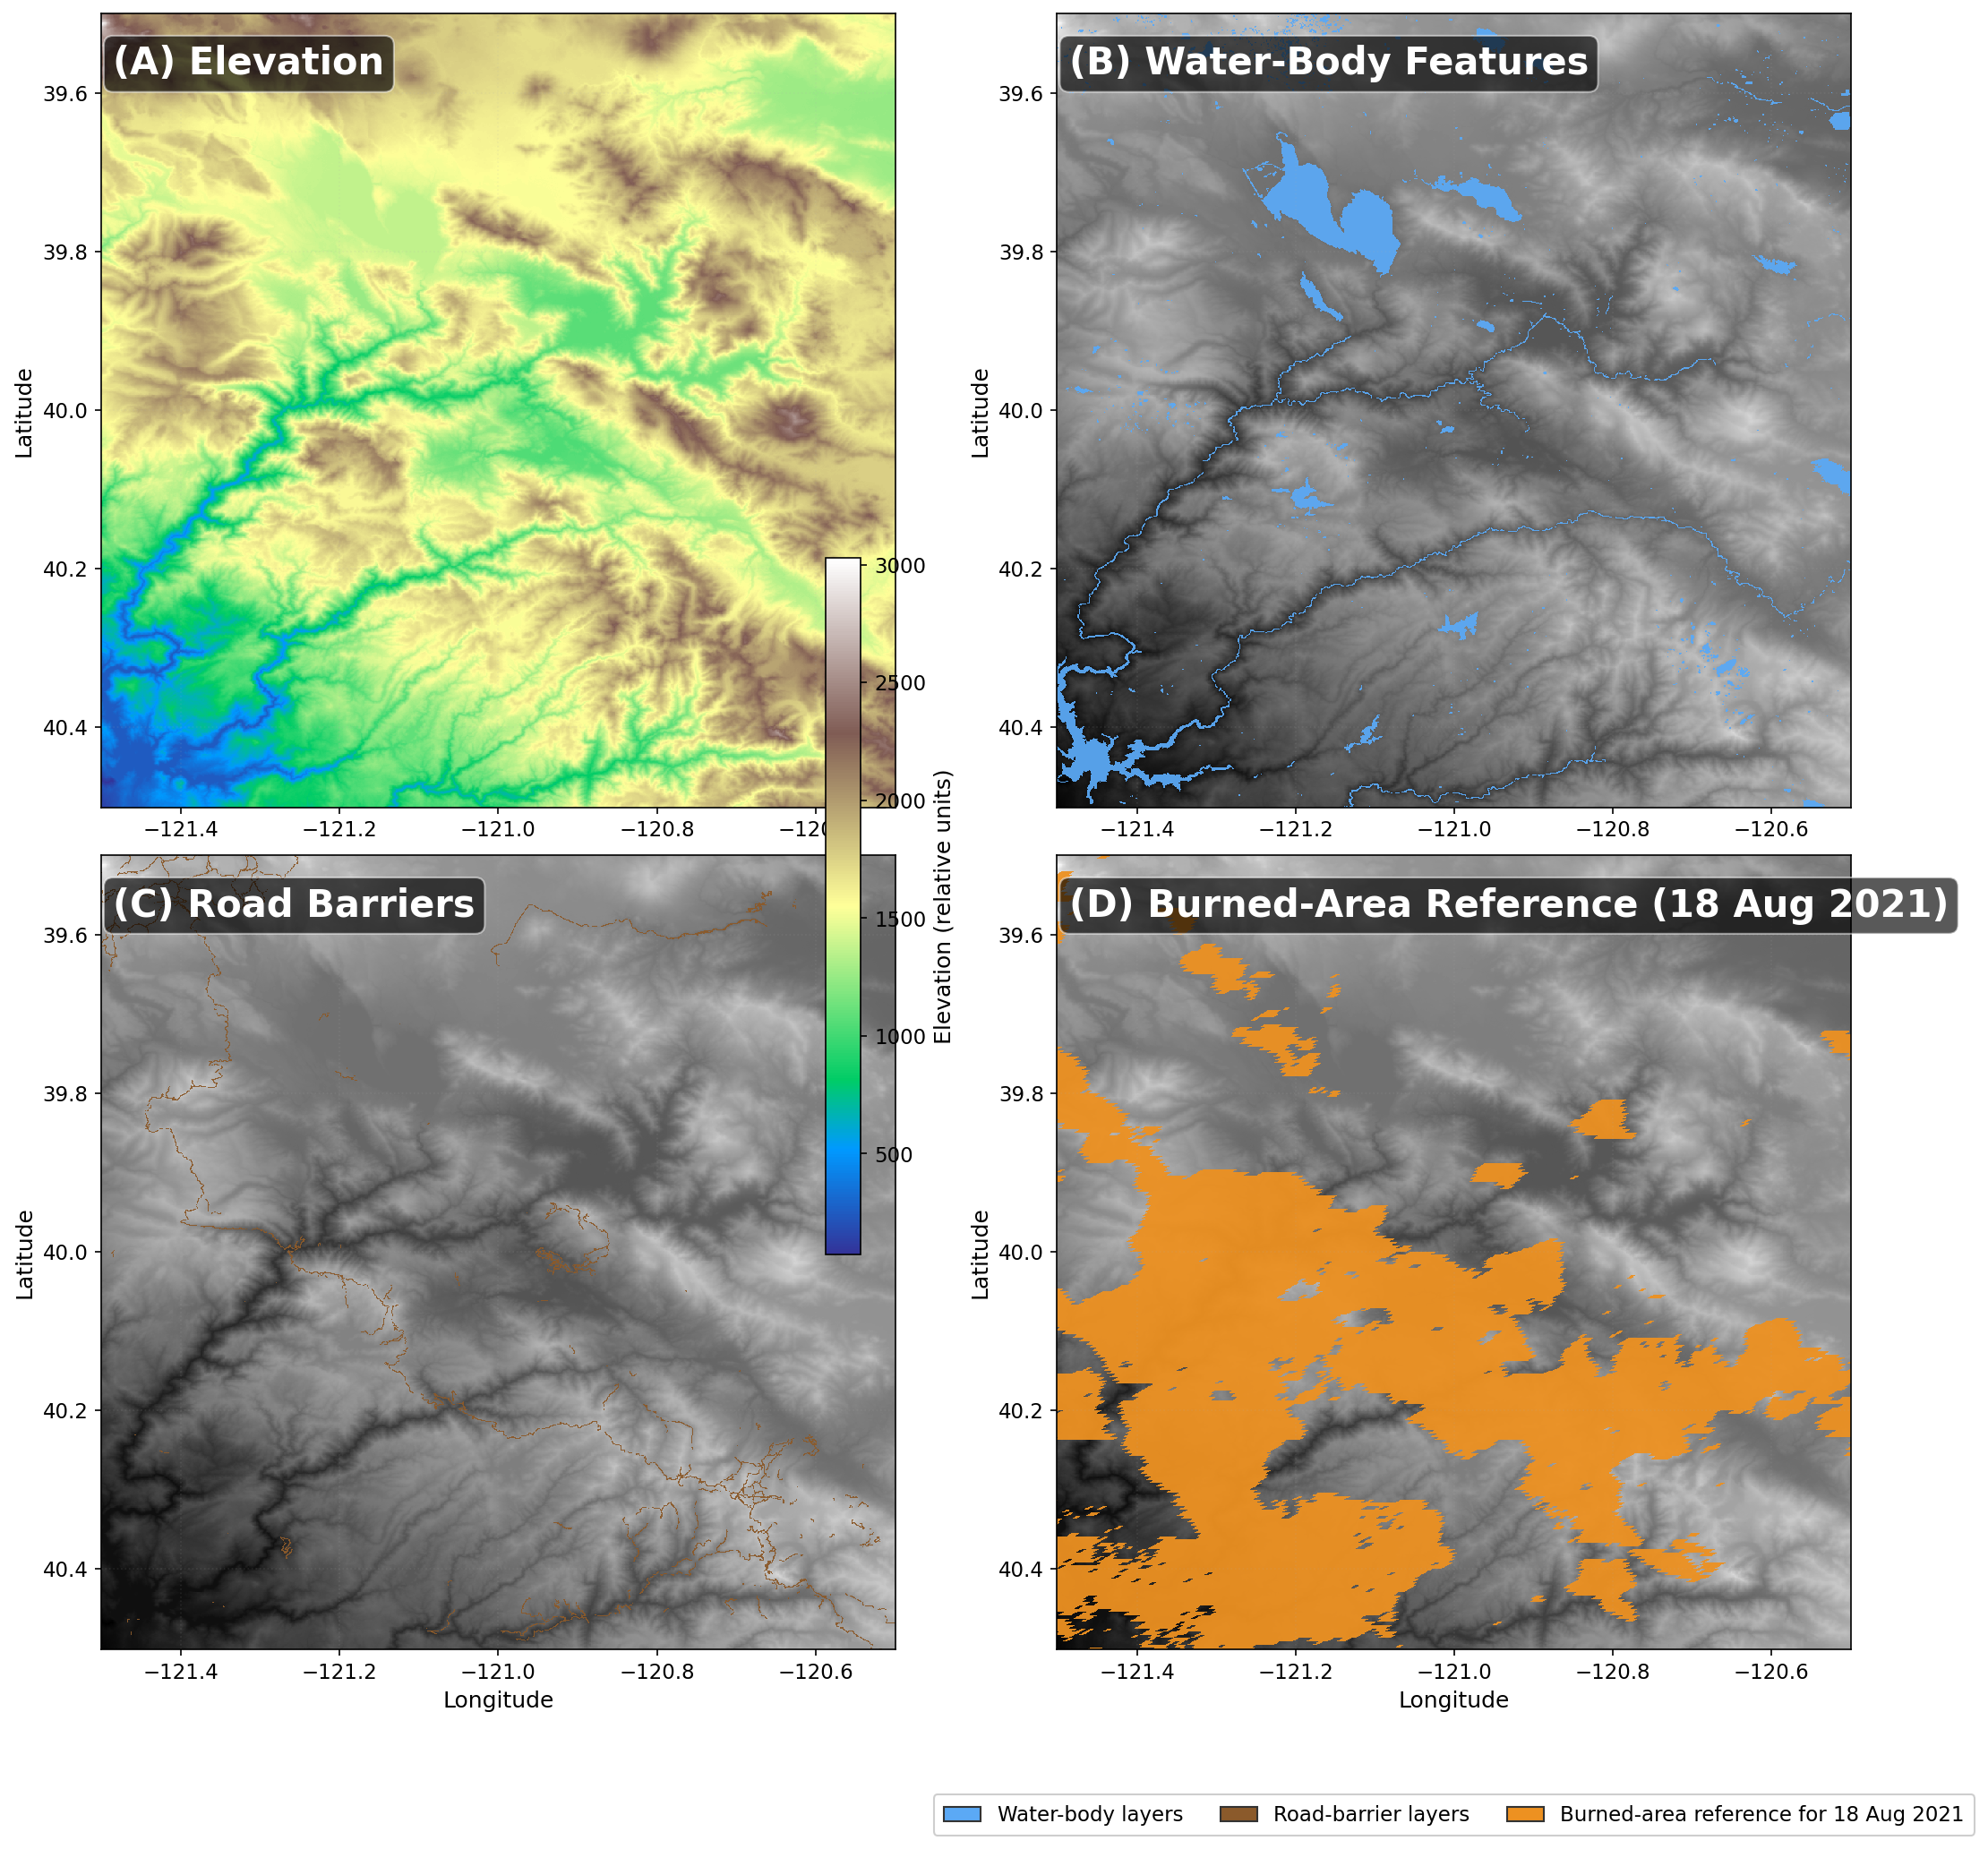
\includegraphics[width=5.9in,height=5.9in]{fig2_spatial_inputs.png}
\captionsetup{hypcap=false}
\captionof{figure}{\textbf{Representative spatial layers used to assemble the Dixie Fire
case-study grid.} (A) Elevation from the DEM used to derive terrain
controls with longitude and latitude axes and a DEM color scale. (B)
Water-body features incorporated into the barrier construction. (C)
Road barriers rasterized onto the common working grid. (D)
Burned-area reference for 18 August 2021 used in the retrospective
evaluation. The bottom legend identifies the binary overlay layers used
in panels (B)--(D).}
\end{minipage}
\else
\begin{figure}[!ht]
\caption{\textbf{Representative spatial layers used to assemble the Dixie Fire
case-study grid.} (A) Elevation from the DEM used to derive terrain
controls with longitude and latitude axes and a DEM color scale. (B)
Water-body features incorporated into the barrier construction. (C)
Road barriers rasterized onto the common working grid. (D)
Burned-area reference for 18 August 2021 used in the retrospective
evaluation. The bottom legend identifies the binary overlay layers used
in panels (B)--(D).}
\end{figure}
\fi

The resulting dataset is therefore a retrospective multi-source daily
stack that combines terrain, vegetation, fuel, barrier, weather, and
observational fire information for one case study. This stack forms the
common input basis for both the baseline cellular automaton and the
hybrid CA+MAS evaluation. Although the prepared dataset spans the full
period from 1 July to 30 September 2021, the quantitative comparison
reported in this manuscript is intentionally restricted to a verified
5-day mid-fire forecasting window from 14 to 18 August 2021, with 14
August used to initialize the forecast state and daily forecast skill
reported for 15 to 18 August.

For clarity, Table 1 summarizes the datasets used to assemble the
case-study stack, together with their native temporal and spatial
resolutions and their roles in the retrospective evaluation.

\begin{longtable}{@{}
  >{\raggedright\arraybackslash}p{0.14\linewidth}
  >{\raggedright\arraybackslash}p{0.21\linewidth}
  >{\raggedright\arraybackslash}p{0.15\linewidth}
  >{\raggedright\arraybackslash}p{0.13\linewidth}
  >{\raggedright\arraybackslash}p{0.20\linewidth}@{}}
\caption{Data sources and roles in the retrospective CA+MAS
case-study dataset.}\label{tab:data_sources}\\
\toprule
\textbf{Dataset} & \textbf{Source} & \textbf{Temporal resolution} &
\textbf{Spatial resolution} & \textbf{Purpose} \\
\midrule
\endfirsthead
\toprule
\textbf{Dataset} & \textbf{Source} & \textbf{Temporal resolution} &
\textbf{Spatial resolution} & \textbf{Purpose} \\
\midrule
\endhead
\bottomrule
\endfoot
DEM, Slope, Aspect & SRTM-derived terrain layers
\cite{earthdata2025b} & Static & 30 to 100 m & Topography \\
Land Cover & ESA WorldCover \cite{worldcover2020} & Static & 10 to
100 m & Fuel proxy baseline \\
NDVI & MODIS MOD13Q1 \cite{earthdata2025a} & 16-day composite & 250 to
100 m & Vegetation condition modifier \\
Burned Area & MODIS MCD64A1 \cite{mcd64a1dataset} & Daily & 500 to 100
m & Retrospective burned-area reference \\
Active Fires & VIIRS VNP14A1 \cite{earthdata2025c} & Daily & 375 to
100 m & Retrospective active-fire guidance \\
Meteorology & ERA5-Land \cite{era5land} & Hourly to daily & 9 km to
100 m & Wind, temperature, humidity, VPD, precipitation \\
Barriers & OpenStreetMap and QGIS
\cite{geofabrik,qgissoftware} & Static & Vector to 100 m & Road and
water-body barriers \\
\end{longtable}

Because the subsequent Methods subsections refer to one verified August
configuration rather than to an abstract parameter space, the key
settings adopted in the reported experiment are listed explicitly in
Table~\ref{tab:verified_parameters}.

\begin{longtable}{@{}
  >{\raggedright\arraybackslash}p{0.28\linewidth}
  >{\raggedright\arraybackslash}p{0.18\linewidth}
  >{\raggedright\arraybackslash}p{0.42\linewidth}@{}}
\caption{Verified August parameter settings used in the retrospective CA+MAS evaluation.}\label{tab:verified_parameters}\\
\toprule
\textbf{Parameter} & \textbf{Value used} & \textbf{Description} \\
\midrule
\endfirsthead
\toprule
\textbf{Parameter} & \textbf{Value used} & \textbf{Description} \\
\midrule
\endhead
\bottomrule
\endfoot
Grid resolution & 100 m & Common raster grid used for all static and daily layers. \\
Grid size & 1115 $\times$ 1115 & DEM-referenced simulation domain. \\
Time step & 1 day & CA update interval and forecast step. \\
Base spread probability $P_0$ & 0.15 & Baseline ignition probability used in the CA component. \\
Number of drones & 5 & Simulated UAV agents in the verified August experiment. \\
Sensing radius & 8 px & Radius of the UAV observation footprint. \\
Movement speed & 35 px/step & Maximum UAV movement per intra-day step. \\
Intra-day update count & 24 & Number of UAV movement and scan steps per simulated day. \\
Burned assimilation radius & 2 px & Neighborhood reinforcement radius around observed burned cells. \\
Clear assimilation radius & 2 px & Neighborhood suppression radius around observed clear cells. \\
\end{longtable}

The following subsections describe how these inputs and parameter
settings enter the preprocessing, spread modeling, observation, and
assimilation stages of the computational experiment.

\subsection*{Preprocessing}

Preprocessing was designed to place all inputs on a common
DEM-referenced raster grid before model execution. The reference DEM
grid in the prepared dataset has dimensions 1115 x 1115 cells, and all
static layers are matched to this shape in the computational
procedure. This alignment step ensures that terrain, fuel, barriers, and
meteorological forcing fields can be used consistently by the cellular
automaton and the hybrid observation-assimilation pipeline.

The preprocessing sequence consisted of four main operations. First,
source rasters were loaded from the prepared geospatial dataset and
truncated or shape-matched to the DEM reference grid when necessary.
Second, NDVI values were clipped to the unit interval before use as a
vegetation-condition modifier. Third, the two barrier rasters
were binarized and merged into one combined barrier mask. After
correction of the previously invalid full-coverage masks, the barrier
layers occupied only a minority of pixels and therefore behaved as
localized spatial constraints rather than domain-wide exclusions.
Fourth, burned-area rasters were converted to daily binary masks, with
positive values denoting cells classified as burned on that day.

In compact form, the preprocessing rules used in the analysis
pipeline can be written as

\begin{equation}
\mathrm{NDVI}^{\ast}(i,j)=\min\left(1,\max\left(0,\mathrm{NDVI}(i,j)\right)\right)
\label{eq:ndvi_clip}
\end{equation}

\begin{equation}
M_{\mathrm{barrier}}(i,j)=\min\left(1,M_{\mathrm{road}}(i,j)+M_{\mathrm{water}}(i,j)\right)
\label{eq:barrier_merge}
\end{equation}

and

\begin{equation}
F_t^{\mathrm{obs}}(i,j)=\mathbf{1}_{\{B_t(i,j)>0\}}
\label{eq:burned_observation}
\end{equation}

where Eqs.~\ref{eq:ndvi_clip}--\ref{eq:burned_observation} define the
three core preprocessing transformations used before model execution.
Here $\mathrm{NDVI}^{\ast}$ is the clipped vegetation-condition layer,
$M_{\mathrm{road}}$ and $M_{\mathrm{water}}$ are the binary road and
water masks rasterized on the DEM grid, $M_{\mathrm{barrier}}$ is the
merged barrier mask, and $F_t^{\mathrm{obs}}$ is the daily binary
burned-area observation derived from the retrospective burned raster
$B_t$.

The daily weather stack was indexed by date and linked to the
burned-area sequence so that each simulation step used a matching set of
meteorological drivers. If an expected daily weather raster was missing,
the preprocessing procedure filled that variable with zeros for the
corresponding day; however, in the assembled Dixie Fire dataset all
required weather variables were available for the full 92-day analysis
window.

This preprocessing procedure yields a unified daily data cube in which
every layer is spatially aligned and available at the same simulation
resolution. For the verified 5-day mid-fire experiment reported in this
manuscript, the corrected combined barrier mask was enabled as a spatial
constraint in both the standalone CA baseline and the CA component of
the hybrid model. The standardized stack is then passed to the
stochastic cellular automaton, the simulated UAV observation module, and
the subsequent binary assimilation step.

\subsection*{Cellular Automaton}

The standalone spread component is a stochastic binary cellular
automaton operating on the daily burned or unburned raster state. Let
$F_t(i,j) \in \{0,1\}$ denote the fire state of cell $(i,j)$ on day $t$,
where $1$ indicates burned and $0$ indicates unburned. A candidate cell
is eligible for ignition only if it is currently unburned and at least
one of its eight neighboring cells is burning.

For eligible cells, the ignition probability is computed as one base
probability multiplied by terrain, fuel, weather, barrier, and
directional correction factors, as summarized in Eq.~\ref{eq:ca_ignition}:

\begin{equation}
P_t(i,j)=P_0 S(i,j) W(i,j) U(i,j) T(i,j) V(i,j) H(i,j) R(i,j) B(i,j) D(i,j) G_t(i,j)
\label{eq:ca_ignition}
\end{equation}

where $P_0=0.15$ is the base spread probability used in the model.
The factors are easier to interpret in groups. Terrain and fuel enter
through the slope factor
$S(i,j)=1+\mathrm{slope}(i,j)/100$ and the normalized fuel factor
$U(i,j)=\mathrm{fuel}(i,j)/\max(\mathrm{fuel})$, so steeper slopes and
more combustible local fuel increase the chance of ignition. Wind and
temperature act as spread amplifiers through
$W(i,j)=1+\mathrm{wind\_speed}(i,j)/10$ and
$T(i,j)=1+0.005\max(T_c(i,j)-20,0)$, which raise the transition
probability under stronger winds and warmer near-surface air. Fuel
dryness and moisture limitation are represented by
$V(i,j)=1+0.02\max(\mathrm{VPD}(i,j),0)$,
$H(i,j)=1/(1+0.01\max(\mathrm{RH}(i,j),0))$, and
$R(i,j)=\exp(-2\max(\mathrm{TP}(i,j),0))$, so high vapor pressure deficit
promotes spread whereas high humidity and precipitation suppress it.

The remaining terms control where spread is allowed and in which
direction it is favored. The barrier term $B(i,j)$ equals $0$ on cells
covered by the combined road or water barrier mask when barriers are
enabled and $1$ otherwise. The wind-direction term $D(i,j)$ increases
the probability by up to 30\% when the local wind direction is aligned
with the neighborhood-derived direction of incoming spread. An optional
multiplicative spread-bias term may also be introduced:

\begin{equation}
G_t(i,j)=\max\left(0,1+g_t(i,j)\right)
\label{eq:spread_bias}
\end{equation}

where Eq.~\ref{eq:spread_bias} defines the optional multiplicative bias
term. The quantity $g_t(i,j)$ is a bounded next-day bias field derived from observed
growth cells, observed frontier burning, and observed clear-growth
regions. When the spread-bias option is disabled, $g_t(i,j)=0$ and the
CA reduces to the base multiplicative form above.

After multiplication, $P_t(i,j)$ is clipped to the interval $[0,1]$ and
the state update is sampled from a Bernoulli trial, so ignition occurs
when a uniform random draw is smaller than $P_t(i,j)$. Burned-area
rasters were binarized by assigning all positive raster values to the
burned class, and no
explicit lightning-ignition term is included in this study. The daily
state is therefore driven by a simple sequence: a cell must have a
burning neighbor, the local multiplicative factors determine its daily
ignition probability, and a Bernoulli draw converts that probability
into the next binary burned or unburned state. This keeps the CA
mathematically explicit while preserving a direct physical reading of
each factor.

\subsection*{Multi-Agent System}

The multi-agent subsystem is implemented as a simulated observation
layer that operates on top of the daily cellular automaton forecast. In
this framework, the number of drones, sensing radius,
movement speed, and intra-day update count are configurable runtime
parameters rather than fixed properties of the method. Each agent stores
its current grid position, sensing radius, movement speed, observed
cells, assigned region, and a day-specific trajectory history that is
later used for reporting and visualization.

These agents should be understood as a proxy for recurring daily aerial
observations within a retrospective forecast-update cycle rather than as
a literal representation of uninterrupted multi-day UAV flight. In this
formulation, each simulated day corresponds to one observation-update
window in which targeted aerial information becomes available before the
next daily forecast step.

For agent $a$, the simulated drone state is represented as
Eq.~\ref{eq:drone_state}:

\begin{equation}
s_t^{(a)}=\left(y_t^{(a)},x_t^{(a)},r^{(a)},v^{(a)}\right)
\label{eq:drone_state}
\end{equation}

where $(y_t^{(a)},x_t^{(a)})$ is the current grid position,
$r^{(a)}$ is the sensing radius, and $v^{(a)}$ is the maximum movement
speed in pixels per intra-day step. If $\mathbf{p}_t^{(a)}$
denotes the current position and $\mathbf{g}_t^{(a)}$ the active target
point, then the implemented movement rule is the bounded directed step
given in Eq.~\ref{eq:drone_motion}:

\begin{equation}
\Delta \mathbf{p}_t^{(a)}=
\min\left(v^{(a)},\left\|\mathbf{g}_t^{(a)}-\mathbf{p}_t^{(a)}\right\|_2\right)
\frac{\mathbf{g}_t^{(a)}-\mathbf{p}_t^{(a)}}{\left\|\mathbf{g}_t^{(a)}-\mathbf{p}_t^{(a)}\right\|_2}
\label{eq:drone_motion}
\end{equation}

followed by clipping to the valid raster domain. When no target is
active, the fallback behavior is a bounded random move on the same grid.

At the start of a run, drones are initialized on burning pixels from the
first available fire-state estimate; if no burning pixels are present,
they are initialized at random grid locations. On each subsequent day,
the simulation design derives candidate observation regions from the predicted
growth field and the forecast fire front, aggregates these cells into
spatial clusters, and ranks the resulting clusters to preserve both
informational value and spatial diversity. Drone-to-region allocation is
then solved as a distance-minimization problem using the Hungarian
algorithm for linear sum assignment \cite{kuhn1955}; a greedy
distance-based rule can be used as a fallback implementation.

The corresponding pairwise assignment cost is the Euclidean distance
between drone and target positions, as given by Eq.~\ref{eq:assignment_cost},

\begin{equation}
c_{ab}=\left\|\mathbf{p}_t^{(a)}-\mathbf{g}_t^{(b)}\right\|_2,
\label{eq:assignment_cost}
\end{equation}

and the Hungarian step selects a one-to-one assignment that minimizes
the total distance across the active drone and target sets. When SciPy
is unavailable, the analysis pipeline falls back to a greedy distance-based
matching rule.

Drone motion is modeled in grid coordinates. When a drone has an
assigned observation region, it follows a short intra-cluster patrol
defined by representative waypoints and advances toward the active
waypoint by at most its configured speed in pixels per intra-day step.
When no explicit assignment is active, the drone moves toward the
nearest currently unexplored informative cell. If no such cell is
available, the drone performs a bounded random move within the grid.

Observations are collected over the swept corridor traced by each drone
during intra-day motion rather than only at waypoint positions. In
practice, the observation set is represented as the union of local
circular sensing footprints sampled along the traversed path. Newly
observed burning cells are written to a shared global observation map
that aggregates all detections made by the simulated agents during the
current daily update cycle.

Accordingly, the observed set for drone $a$ over one daily update window
can be summarized by Eq.~\ref{eq:observed_support}:

\begin{equation}
O_t^{(a)}=\bigcup_{k=0}^{K_t^{(a)}} \left\{(i,j):
\left\|(i,j)-\mathbf{p}_{t,k}^{(a)}\right\|_2 \le r^{(a)}\right\}
\label{eq:observed_support}
\end{equation}

where $\mathbf{p}_{t,k}^{(a)}$ are the sampled intra-day positions along
the path of the drone. The global observation support used by the
assimilation step is then $K_t=\bigcup_a O_t^{(a)}$.

In this formulation, the MAS does not replace the spread model and
does not perform obstacle-aware route planning. Its role is to
concentrate simulated observations on informative fire-front regions and
to provide a compact, reproducible mechanism for retrospective sensing
within the hybrid CA+MAS framework.

For reproducibility, the framework exposes the CA base spread
probability, drone count, sensing radius, movement speed, intra-day
update count, targeting strategy, assignment rule, spread-bias toggle,
and assimilation radii as explicit runtime parameters. The manuscript
results reported here correspond to one verified August parameter set,
summarized in Table~\ref{tab:verified_parameters}, rather than to
generic default settings.

\subsection*{Data Assimilation}

Data assimilation is implemented as a lightweight binary
state-correction step rather than as an Ensemble Kalman Filter or a
Particle Filter \cite{evensen2003,doucet2001}. Because the fire map is
represented as a binary burned or unburned raster, the assimilation
logic operates directly on binary cell states and therefore remains
consistent with the underlying cellular automaton representation.

After the intra-day drone motion and scanning steps are completed, the
evaluation protocol copies the current CA prediction and applies a confirm-deny
update on all cells present in the shared global observation map. For each
observed location, the corrected fire map is set to 1 when the
retrospective burned reference indicates fire presence and to 0
otherwise. In this way, confirmed ignitions are inserted into the model
state and false activations are removed before the next daily CA spread
step is executed.

Let $F_t^{\mathrm{pred}}$ denote the daily CA prediction before
assimilation, let $F_t^{\mathrm{ref}}$ denote the retrospective burned
reference used during replay, and let $K_t$ denote the union of cells
observed by all drones during that day. The implemented binary
correction operator is given in Eq.~\ref{eq:binary_assim}:

\begin{equation}
\widetilde{F}_t(i,j)=
\begin{cases}
1, & (i,j)\in K_t \text{ and } F_t^{\mathrm{ref}}(i,j)=1, \\
0, & (i,j)\in K_t \text{ and } F_t^{\mathrm{ref}}(i,j)=0, \\
F_t^{\mathrm{pred}}(i,j), & (i,j)\notin K_t.
\end{cases}
\label{eq:binary_assim}
\end{equation}

Thus, observation-supported burned cells are confirmed, observation-supported
false positives are removed, and unobserved cells retain the CA state
predicted for that day.

In the present formulation, this direct cellwise update
is then extended to small local neighborhoods around observed burned and
observed clear cells using configurable dilation radii. Burned
observations therefore reinforce nearby frontier and growth pixels,
whereas clear observations suppress nearby false activations. The core
confirm-deny logic of Eq.~\ref{eq:binary_assim} is preserved, but the
effective update is slightly more spatially permissive than a purely
pointwise overwrite.

The corrected map is then passed to the CA spread operator to generate
the next hybrid forecast. In parallel, the evaluation procedure also propagates an
uncorrected CA state for comparison purposes. This produces a day-by-day
paired evaluation in which the hybrid forecast and the baseline CA
forecast can be scored against the same retrospective burned-area target
while sharing the same meteorological forcing and barrier configuration.

If $\Phi(\cdot;\theta_t)$ denotes the CA transition operator under the
weather and static inputs for day $t$, then the hybrid and baseline
forecast branches can be summarized as in Eq.~\ref{eq:forecast_branches}:

\begin{equation}
F_{t+1}^{\mathrm{hyb}}=\Phi\left(\widetilde{F}_t;\theta_t\right),
\qquad
F_{t+1}^{\mathrm{base}}=\Phi\left(F_t^{\mathrm{pred}};\theta_t\right)
\label{eq:forecast_branches}
\end{equation}

This notation makes explicit that the only difference between the two
branches is the insertion of the binary observation-correction step
before the next daily CA propagation.

This assimilation design has two practical consequences. First, it is
computationally lightweight because it avoids solving any
high-dimensional inverse problem. Second, it remains interpretable
because every correction corresponds to an explicit cell-level
observation supplied by the simulated drone layer. For the present
retrospective case study, this simple binary confirm-deny rule is
sufficient to test whether targeted observations improve short-horizon
wildfire-front reconstruction.

The same observed footprint can also be used to
blend the daily weather fields locally before the next forecast step.
If $X_t^{\mathrm{prior}}$ and $X_t^{\mathrm{sens}}$ denote the prior and
sensor-derived weather rasters for a given variable and
$\Omega_t^{\mathrm{obs}}$ denotes the dilated observed footprint, then
the local weather update is given by Eq.~\ref{eq:weather_assim}:

\begin{equation}
X_t^{\mathrm{assim}}(i,j)=
\begin{cases}
(1-\lambda_w)X_t^{\mathrm{prior}}(i,j)+\lambda_w X_t^{\mathrm{sens}}(i,j), & (i,j)\in \Omega_t^{\mathrm{obs}}, \\
X_t^{\mathrm{prior}}(i,j), & (i,j)\notin \Omega_t^{\mathrm{obs}},
\end{cases}
\label{eq:weather_assim}
\end{equation}

with blend weight $\lambda_w\in[0,1]$. This local meteorological update
is auxiliary: it complements rather than replaces the primary binary
confirm-deny correction of the fire-state raster.



\section*{Results}

The study results demonstrate that the proposed method improves
short-horizon fire-front reconstruction relative to the baseline
cellular automaton. In the retrospective hybrid framework, drone
trajectories remain concentrated near active and previously unobserved
burning regions, which increases the coverage of informative fire-front
segments during the simulated observation stage (Fig 3).

\iflocalfigurepreview
\begin{minipage}{\linewidth}
\centering
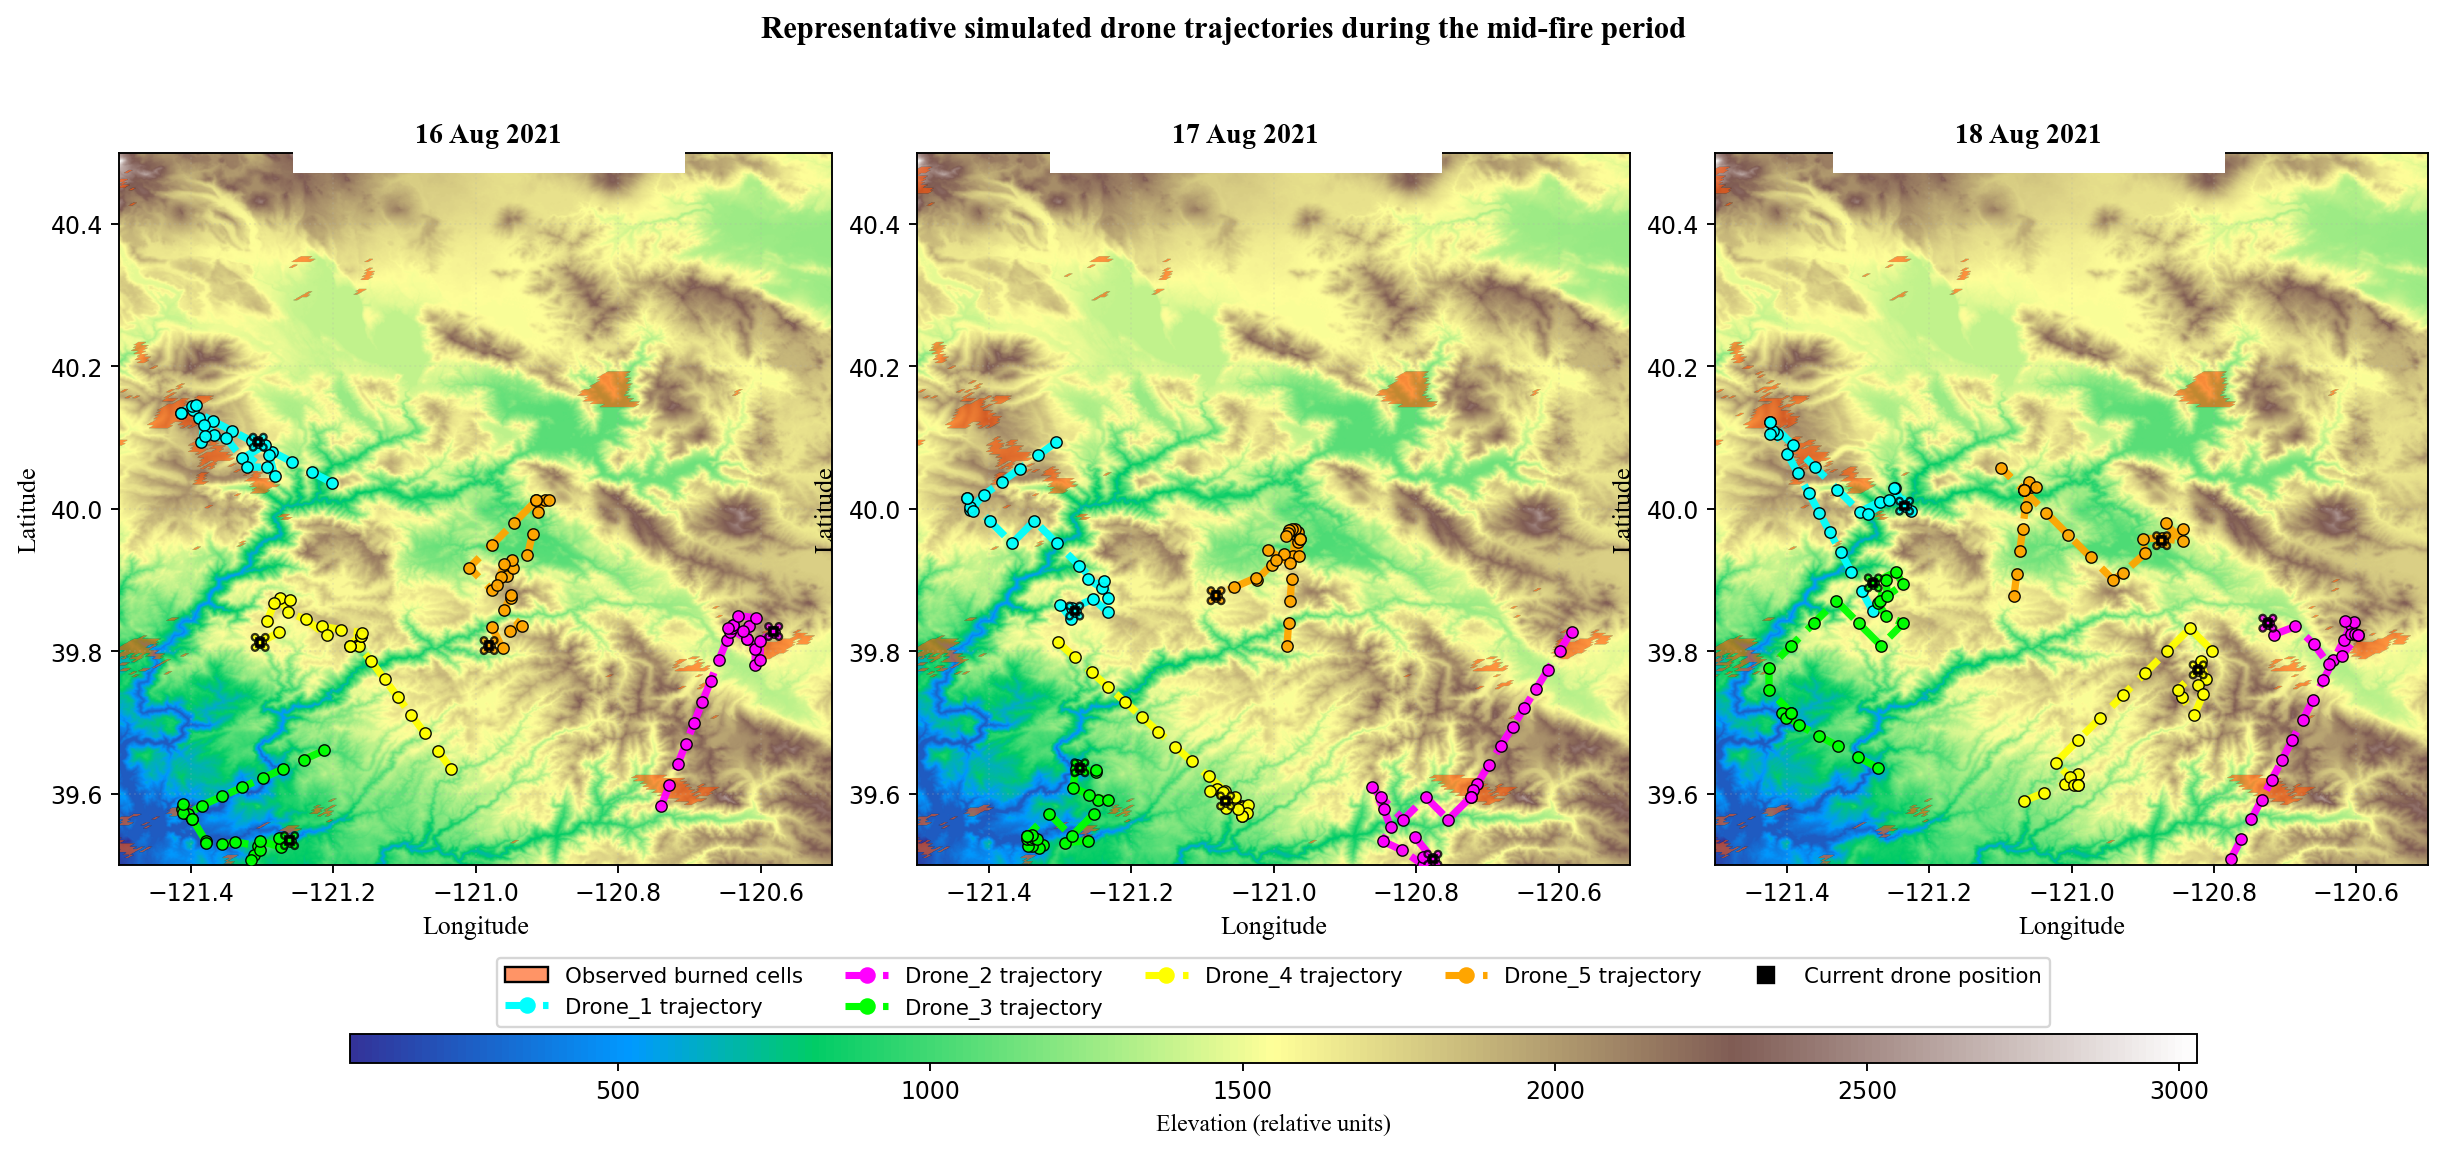
\includegraphics[width=5.8in]{fig3_drone_trajectories.png}
\captionsetup{hypcap=false}
\captionof{figure}{\textbf{Composite view of representative simulated drone trajectories
during the middle portion of the retrospective fire period.}
(a) 16 August 2021, (b) 17 August 2021, and (c) 18 August 2021. Orange polygons
denote observed burned cells, colored dashed lines denote individual
drone trajectories, square markers denote current drone positions, and
the DEM background provides terrain context for each daily observation
cycle.}
\end{minipage}
\else
\begin{figure}[!ht]
\caption{\textbf{Composite view of representative simulated drone trajectories
during the middle portion of the retrospective fire period.}
(a) 16 August 2021, (b) 17 August 2021, and (c) 18 August 2021. Orange polygons
denote observed burned cells, colored dashed lines denote individual
drone trajectories, square markers denote current drone positions, and
the DEM background provides terrain context for each daily observation
cycle.}
\end{figure}
\fi

Across successive daily update cycles, the simulated observation layer
remains concentrated near active fire-front segments, providing dense
localized coverage where state correction is most informative. This
adaptive sensing pattern is visible in the hybrid configuration. The later dates shown in Fig 3 also provide a
clearer visual demonstration of how the agents redistribute as the
front evolves across the verified window.

To quantitatively evaluate the contribution of the multi-agent subsystem
to modeling accuracy, a comparative analysis was conducted between the
baseline CA and the hybrid CA+MAS architecture incorporating drone
observations.

The simulated observation policy redirects sensing effort across the
retrospective experiment as fire-front geometry changes, while coverage
remains concentrated near active segments.

For the adopted 5-day evaluation window from 14 to 18 August 2021, with
corrected road and water barrier masks enabled in the CA component, the
standalone baseline CA achieved a mean Intersection over Union (IoU) of
0.6664, whereas the hybrid CA+MAS configuration reached 0.6992. This
corresponds to an absolute IoU gain of 0.0328, indicating that the
assimilation of simulated aerial observations improved short-horizon
wildfire-front reconstruction over the barrier-aware baseline forecast
(Table~\ref{tab:summary_metrics}).

{% pandoc longtable wrapper
\begin{longtable}[]{@{}
  >{\centering\arraybackslash}p{(\linewidth - 6\tabcolsep) * \real{0.3633}}
  >{\centering\arraybackslash}p{(\linewidth - 6\tabcolsep) * \real{0.1817}}
  >{\centering\arraybackslash}p{(\linewidth - 6\tabcolsep) * \real{0.2276}}
  >{\centering\arraybackslash}p{(\linewidth - 6\tabcolsep) * \real{0.2275}}@{}}
\caption{Comparative summary of mean Intersection over Union (IoU) for the standalone CA baseline and the CA+MAS hybrid configuration.}\label{tab:summary_metrics}\\
\toprule\noalign{}
\endhead
\bottomrule\noalign{}
\endlastfoot
\textbf{Model Variant} & \textbf{Mean IoU} & \textbf{Absolute Gain} &
\textbf{Relative Gain} \\
CA (Cellular Automaton only) & 0.6664 & -- & -- \\
CA+MAS (with drone feedback) & 0.6992 & +0.0328 & +4.92\% \\
\end{longtable}
}

Because the revised comparison is intentionally limited to the verified
5-day experiment, we report only those summary metrics that are directly
reproduced by the reproducible evaluation protocol. In addition to the higher
mean IoU, the hybrid run yielded a mean F1 score of 0.8229 compared with
0.7998 for the standalone baseline CA, which is consistent with the
visual improvement shown in the comparative figures.

Across the evaluated forecast days, the hybrid CA+MAS system yields
higher IoU and F1 than the standalone cellular automaton, as summarized
in Table~\ref{tab:daily_metrics}. The mean IoU improvement for this
5-day experiment is +0.0328 (from 0.6664 to 0.6992), corresponding to a
relative increase of +4.92 \%, while the mean F1 score increases from
0.7998 to 0.8229. Positive daily IoU gains are observed on every
evaluated day of the verified window.

{% pandoc longtable wrapper
\begin{longtable}[]{@{}
  >{\centering\arraybackslash}p{(\linewidth - 12\tabcolsep) * \real{0.17}}
  >{\centering\arraybackslash}p{(\linewidth - 12\tabcolsep) * \real{0.14}}
  >{\centering\arraybackslash}p{(\linewidth - 12\tabcolsep) * \real{0.14}}
  >{\centering\arraybackslash}p{(\linewidth - 12\tabcolsep) * \real{0.13}}
  >{\centering\arraybackslash}p{(\linewidth - 12\tabcolsep) * \real{0.14}}
  >{\centering\arraybackslash}p{(\linewidth - 12\tabcolsep) * \real{0.14}}
  >{\centering\arraybackslash}p{(\linewidth - 12\tabcolsep) * \real{0.14}}@{}}
\caption{Daily and mean performance comparison between the standalone
CA baseline and the CA+MAS hybrid configuration over the verified
evaluation window. The 14 August 2021 raster is used as the
initialization state; therefore, daily forecast metrics are reported for
15 to 18 August 2021.}\label{tab:daily_metrics}\\
\toprule\noalign{}
\endhead
\bottomrule\noalign{}
\endlastfoot
\textbf{Date} & \textbf{IoU CA} & \textbf{IoU Hybrid} & \textbf{$\Delta$ IoU} & \textbf{F1 CA} & \textbf{F1 Hybrid} & \textbf{$\Delta$ F1} \\
20210815 & 0.6670 & 0.6818 & +0.0148 & 0.8003 & 0.8108 & +0.0105 \\
20210816 & 0.6731 & 0.7037 & +0.0305 & 0.8046 & 0.8261 & +0.0214 \\
20210817 & 0.6690 & 0.7080 & +0.0390 & 0.8017 & 0.8290 & +0.0274 \\
20210818 & 0.6563 & 0.7032 & +0.0470 & 0.7925 & 0.8258 & +0.0333 \\
\textbf{Mean} & \textbf{0.6664} & \textbf{0.6992} & \textbf{+0.0328} & \textbf{0.7998} & \textbf{0.8229} & \textbf{+0.0232} \\
\end{longtable}
}

Fig 4 presents a spatial comparison for
the final evaluated day of the verified window (18 August 2021), showing:

(a) the observed burned-area reference;

(b) the forecast produced by the standalone cellular automaton (CA)
baseline; and

(c) the forecast generated by the hybrid CA+MAS model after correction
with the simulated daily aerial observation layer.

The visual comparison places the observed burned-area reference, the
standalone CA baseline forecast, and the hybrid CA+MAS forecast side by
side for the same final evaluated day.

\iflocalfigurepreview
\begin{minipage}{\linewidth}
\centering
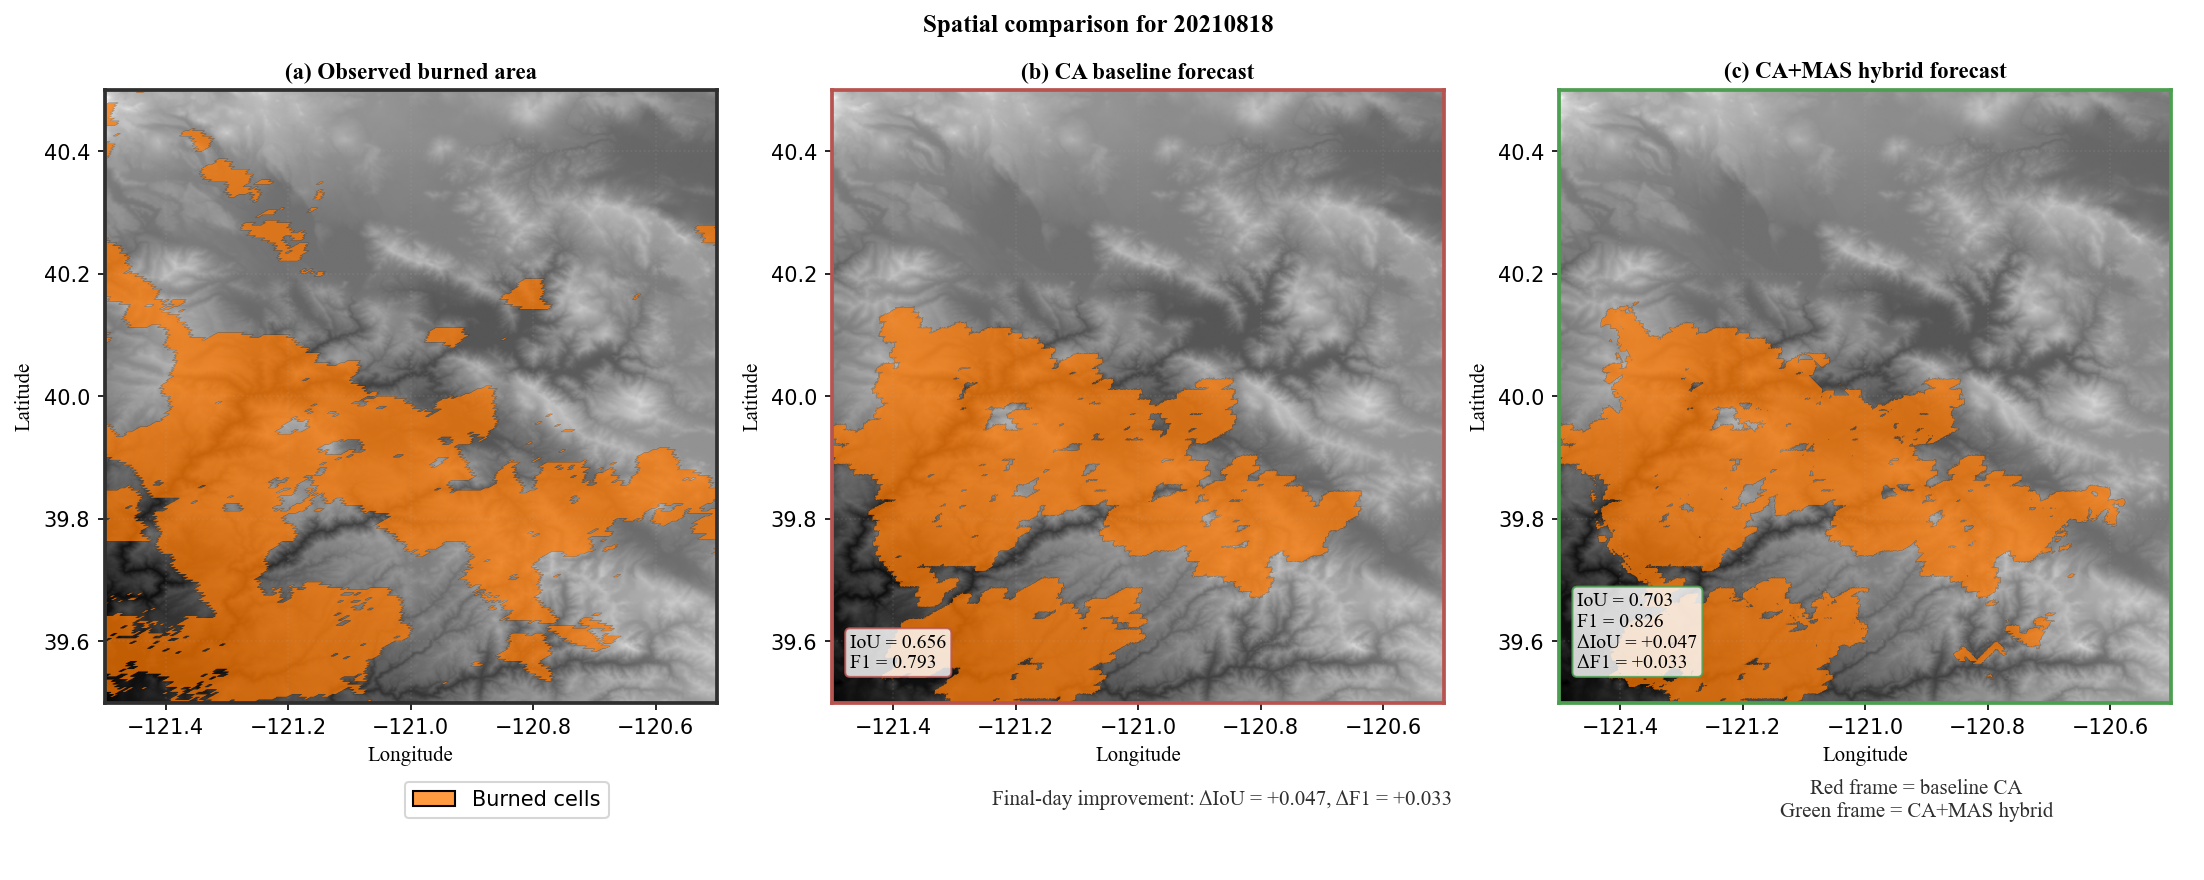
\includegraphics[width=6.0in,height=3.8in,keepaspectratio]{fig4_spatial_comparison.png}
\captionsetup{hypcap=false}
\captionof{figure}{\textbf{Spatial comparison on 18 August 2021
between the observed burned-area reference, the standalone CA baseline
forecast, and the CA+MAS hybrid forecast corrected by the simulated
daily aerial observation layer.} The numerical annotations within panels
(b) and (c) report final-day IoU and F1 values for 18 August 2021,
whereas the summary values discussed in Table~\ref{tab:summary_metrics} and Table~\ref{tab:daily_metrics} correspond to
means aggregated across the full verified evaluation window.}
\end{minipage}
\else
\begin{figure}[!ht]
\caption{\textbf{Spatial comparison on 18 August 2021
between the observed burned-area reference, the standalone CA baseline
forecast, and the CA+MAS hybrid forecast corrected by the simulated
daily aerial observation layer.} The numerical annotations within panels
(b) and (c) report final-day IoU and F1 values for 18 August 2021,
whereas the summary values discussed in Table~\ref{tab:summary_metrics} and Table~\ref{tab:daily_metrics} correspond to
means aggregated across the full verified evaluation window.}
\end{figure}
\fi

Taken together, the spatial comparison and tabulated metrics describe
the same verified short-horizon evaluation window.

\section*{Discussion}

The verified 5-day mid-fire experiment indicates that the hybrid CA--MAS
configuration improves short-horizon wildfire-front reconstruction
because the forecast state is corrected before errors can accumulate
across successive daily steps. In the present framework, the gain
does not arise from a more complex spread model, but from inserting
targeted simulated observations into the daily forecast-update cycle.
This makes the observed improvement mechanistically consistent with the
simulation design: the CA provides an interpretable baseline
forecast, the MAS concentrates attention on informative front segments,
and the binary assimilation rule removes false activations while
restoring missed burned cells.

Classical cellular automata models \cite{freire2019,schumaker2022} lack intrinsic mechanisms for adapting to changing
conditions once a forecast has been initialized. In contrast, the
proposed CA+MAS system incorporates an explicit forecast-observe-correct
loop driven by targeted simulated UAV observations. This architecture
improves the suitability of the model for short-horizon updating when
wind, fuel, and vegetation conditions cause the fire front to evolve
rapidly.

In comparison with physical--mathematical advection--diffusion--reaction
(ADR) models \cite{navasmontilla2025}, the CA+MAS framework
operates on aggregated input layers and is readily scalable to large
spatial domains. This contrast is relevant to the present results
because the observed IoU improvement was obtained without introducing a
high-parameter physical solver; instead, the improvement emerged from a
computationally lightweight correction loop applied to the same daily
forcing and barrier-aware CA backbone. The current case study therefore
suggests that, for short retrospective windows, targeted observation and
state correction can yield useful accuracy gains even within a simpler
spread-modeling framework.

Deep neural network architectures, including CNNs, convolutional long
short-term memory (ConvLSTM) networks, and transformers, have demonstrated high predictive accuracy for fire
dynamics based on satellite observations \cite{andrianarivony2024,marjani2023}. However, these
approaches typically require large volumes of labeled training data,
offer limited interpretability, and exhibit reduced generalizability
when applied to previously unseen regions without additional retraining.
In contrast, the CA+MAS framework retains physically interpretable
parameters, operates independently of training datasets, and supports
explicit state updating through the simulated observation layer.

A key distinguishing feature of the hybrid architecture is the explicit
use of targeted observations and shared observation-map assimilation
within a lightweight CA framework. Although wildfire
forecasting studies have also explored latent data assimilation and
satellite-based fire-growth updates \cite{cheng2022,chen2022,mcclure2023},
the present model avoids solving a high-dimensional filtering problem.
Instead, it uses a simulated daily aerial observation layer to correct
missed burning cells and suppress false activations before the next
spread step. This design helps explain why the model performs best in a
short-horizon retrospective setting: corrections are local,
interpretable, and directly tied to the same cells that drive the next
daily forecast update.

The modular architecture of the system enables straightforward expansion
of its functional capabilities. Potential extensions include the
incorporation of multi-agent reinforcement learning algorithms for
autonomous swarm coordination, the integration of higher-resolution
meteorological models, and embedding within broader
situational-awareness pipelines. These extensions are motivated by the
current findings rather than independent of them: because the verified
case study supports the value of targeted observation and explicit state
correction, future work should focus on improving where, when, and how
those observations are generated rather than on broadening the claims of
the present study. In its current form, the CA+MAS framework should be
understood as an interpretable and extensible prototype for wildfire
monitoring and forecasting rather than as a fully operational end-to-end
deployment.

\subsection*{Limitations}

Several limitations should be stated explicitly. First, the present
evaluation is based on a single retrospective case study and a verified
5-day mid-fire window, so the reported gains should not yet be treated
as evidence of broad cross-fire generalization. Second, the aerial
component is represented by simulated UAV observations rather than by a
historical deployment log, which means that sensing coverage, movement,
and correction timing were assessed within a computational experiment
rather than under operational field constraints. Third, the
data-assimilation module is intentionally simple: it applies explicit
binary state correction and local neighborhood dilation, but it does not
estimate posterior uncertainty or solve a higher-dimensional filtering
problem. Fourth, although the verified August parameter set is now
reported explicitly, the present manuscript does not claim that this
parameterization is optimal outside the evaluated setting. These limits
do not invalidate the present findings, but they define the scope within
which the reported improvements should be interpreted.

\section*{Conclusions and future directions}

A hybrid architecture for wildfire modeling and forecasting has been
developed by integrating a cellular automaton (CA) with a simulated
drone-based multi-agent system (MAS). The model operates through an adaptive
closed-loop sequence comprising CA simulation, MAS-driven observation,
data assimilation, and state update. In the verified 5-day evaluation
window from 14 to 18 August 2021, with corrected barrier masks enabled
in the CA component, this integrated approach increased mean IoU from
0.6664 for the standalone baseline CA to 0.6992 for the hybrid
configuration, while the mean F1 score increased from 0.7998 to 0.8229.
These results indicate that spatially targeted recurrent aerial
observations can improve short-horizon wildfire-front forecasting.

The model offers high interpretability, linear scalability, and a
comparatively lightweight update mechanism. Compared with alternatives
such as FARSITE, deep learning-based approaches, and EnKF-style filters,
it requires fewer computational resources, adapts its state through
explicit observations, and preserves physical consistency in the
forecast-update loop.

The present retrospective results suggest that the developed approach
can inform future decision-support and situational-awareness frameworks
for wildfire management. Its modularity and
transparency make it suitable for further experimentation across
additional regions and scenario types, provided that the present study
is understood as a retrospective evaluation of simulated daily aerial
observations rather than as a direct operational deployment study.

Future work may extend the hybrid architecture through the
integration of machine learning and reinforcement learning techniques.
In particular, the multi-agent UAV subsystem may evolve from
deterministic task allocation toward adaptive behaviors derived from
multi-agent reinforcement learning (MARL) algorithms, enabling drones to
autonomously optimize routes, observation priorities, and operational
strategies under uncertainty. Another avenue involves employing ML
models for the dynamic calibration of cellular automaton parameters,
including fuel-proxy scaling, wind and humidity adjustment terms,
precipitation damping, and daily state-transition probabilities. These
enhancements may strengthen
forecast robustness and support the development of a more adaptive
forecast--observe--learn cycle, thereby improving predictive accuracy
and the flexibility of future wildfire-modeling frameworks.

\section*{Data Availability Statement}
The original input datasets used in this study are publicly available from the repositories listed in Table~\ref{tab:data_sources}. Processed intermediate files are available from the corresponding author upon reasonable request.

\section*{Code Availability Statement}
The simulation scripts used to generate the reported results are available from the corresponding author upon reasonable request.

\section*{Funding Statement}
The authors received no specific funding for this work.

\section*{Competing Interests}
The authors declare that they have no competing interests.

\section*{Acknowledgments}

The authors have no additional acknowledgments to report.

\nolinenumbers

\bibliography{wildfire_references}

\end{document}
